\documentclass[a4paper,12pt]{article}
\usepackage{longtable}
\usepackage{tabularx}
\usepackage{tabularray}
\usepackage[table,xcdraw]{xcolor}
\usepackage{graphicx}
\usepackage[export]{adjustbox}
\usepackage{amsmath} % for the equation* environment
\usepackage[hmargin=2.5cm, vmargin={3cm,3cm}, a4paper]{geometry} 
\usepackage{amsmath,amssymb,amsthm,mathrsfs}
\setlength{\headheight}{12pt}
\usepackage{listings}
\usepackage{xcolor}
\usepackage{float} % Provides the H float modifier option for better float positioning
\usepackage{hyperref}
\usepackage{geometry}
\geometry{a4paper, margin=1in}
\usepackage{array}
\usepackage{ragged2e} % Para justificar el texto

\definecolor{codegreen}{rgb}{0,0.6,0}
\definecolor{codegray}{rgb}{0.5,0.5,0.5}
\definecolor{codepurple}{rgb}{0.58,0,0.82}
\definecolor{backcolour}{rgb}{0.95,0.95,0.92}

\lstdefinestyle{mystyle}{
    backgroundcolor=\color{backcolour},   
    commentstyle=\color{codegreen},
    keywordstyle=\color{blue},
    numberstyle=\tiny\color{codegray},
    stringstyle=\color{codepurple},
    basicstyle=\ttfamily\footnotesize,
    breakatwhitespace=false,
    breaklines=true,
    captionpos=b,
    keepspaces=true,
    numbers=left,
    numbersep=5pt,
    showspaces=false,
    showstringspaces=false,
    showtabs=false,
    tabsize=2
}

\hypersetup{
  colorlinks = true, % enables coloring of links
  linkcolor = black, % sets link color to white
  citecolor = black, % sets citation links color to white
  filecolor = black, % sets file links color to white
  urlcolor = blue   % sets URL links color to white
}

\lstset{style=mystyle}



\title{SDS\_FinalProject}
\author{Alex Romano \& Dand Marbà \& Oriol Miranda}
\date{07/06/2024}

\begin{document}

\maketitle
\newpage
\tableofcontents
\newpage

% Introduction
\section{Introduction}
This report describes the development and implementation of a software-defined network (SDN). The main objective is to demonstrate how to use Mininet and the Ryu controller to efficiently manage a network, including security and monitoring functionalities.

% Background and Motivation
\section{Background and Motivation}
The rapid evolution of networking technologies has led to the development of Software-Defined Networking (SDN) as a means to enhance network flexibility and manageability. Traditional network architectures are often rigid and difficult to manage, especially in large-scale environments. SDN decouples the control plane from the data plane, enabling centralized network management and programmability.

This project aims to explore the capabilities of SDN using Mininet and the Ryu controller. The primary motivation is to implement and test key network functionalities such as load balancing, firewall, and network monitoring in a simulated environment. By integrating tools like Snort for intrusion detection and Grafana for performance metrics visualization, this project seeks to demonstrate the advantages of SDN in terms of security and efficiency.

\section{Project Description}
This project focuses on the creation and management of a software-defined network (SDN) using Mininet and the Ryu controller. The network is designed to simulate a realistic environment, implementing several key functionalities and integrating various tools to enhance performance, security, and monitoring capabilities. The primary components and tools used in this project include:

\begin{itemize}
    \item \textbf{SDN-based Network:} The foundation of the project is a software-defined network that allows for centralized control and dynamic configuration of network elements.
    \item \textbf{Simulation Environment: Mininet} Mininet is used to simulate the network topology, providing a platform to test and develop SDN applications in a controlled environment.
    \item \textbf{Controller: RYU} The Ryu controller is employed to manage the SDN, implementing control logic for various network functionalities such as switching, firewall rules, and load balancing.
    \item \textbf{Load Balancer:} A load balancer is implemented to distribute network traffic evenly across multiple servers, optimizing resource utilization and improving network performance.
    \item \textbf{Intrusion Detection System (IDS): Snort} Snort is integrated into the network to monitor traffic for suspicious activities and potential security threats.
    \item \textbf{Attack Generator: hping3} The hping3 tool is used to simulate different types of network attacks, allowing for testing and validation of the network's security mechanisms.
    \item \textbf{Monitoring and Visualization: Grafana} Grafana, in combination with Telegraf, is used to monitor network performance metrics and visualize data, providing insights into network health and behavior.
\end{itemize}

\begin{figure}[h]
    \centering
    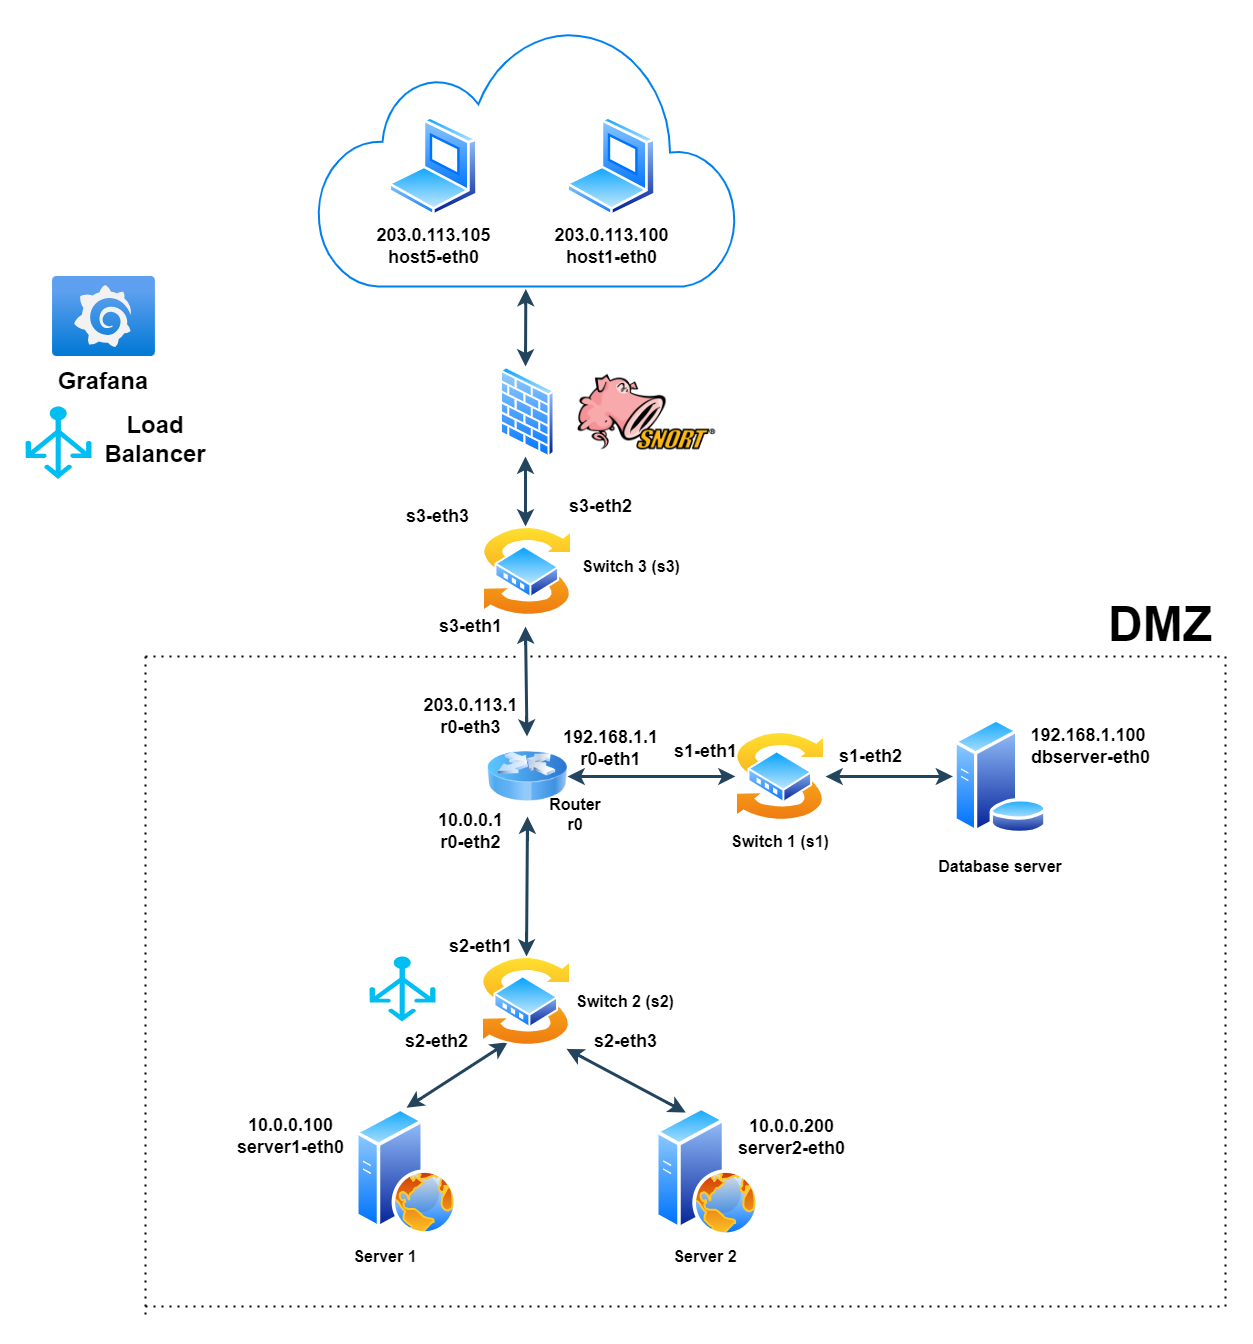
\includegraphics[width=0.9\textwidth]{1.png}
    \caption{Network Topology and Components}
    \label{fig:network_topology}
\end{figure}

The network topology (see Figure \ref{fig:network_topology}) is structured to simulate a typical enterprise network with the following components:

\begin{itemize}
    \item \textbf{Hosts:} Two hosts (\texttt{203.0.113.105} and \texttt{203.0.113.100}) represent external devices connecting to the network.
    \item \textbf{Switches:} Three switches (\texttt{s1}, \texttt{s2}, \texttt{s3}) are used to manage data traffic within the network.
    \item \textbf{Router:} A router (\texttt{r0}) connects different segments of the network, facilitating communication between them.
    \item \textbf{Servers:} Two servers (\texttt{10.0.0.100} and \texttt{10.0.0.200}) are deployed to handle application workloads and are load-balanced to optimize performance.
    \item \textbf{Database Server:} A database server (\texttt{192.168.1.100}) is placed in the DMZ (Demilitarized Zone) to handle sensitive data transactions securely.
    \item \textbf{Snort IDS:} Snort is configured to monitor traffic between the external hosts and the internal network, providing real-time intrusion detection.
    \item \textbf{Grafana Monitoring:} Grafana is set up to collect and visualize network performance metrics, integrating with Telegraf for data collection.
\end{itemize}

The design and implementation of this SDN project aims to demonstrate the benefits of SDN in terms of network flexibility, security, and performance monitoring. The integration of various tools and functionalities highlights the potential of SDN to manage and secure modern network infrastructures effectively.



\section{Implementation}

The implementation of the SDN project involves several scripts that configure and manage different aspects of the network. Below, we detail the functionality and configuration of each script used in this project.

\subsection{RYU Controller}

\subsubsection{snort.py}
The \texttt{snort.py} script integrates the Snort Intrusion Detection System (IDS) with the Ryu controller. This script configures Snort to monitor network traffic for potential threats and anomalies. The integration with Ryu allows Snort to send alerts to the controller, which can then take appropriate actions, such as blocking malicious traffic.

\begin{verbatim}
from ryu.base import app_manager
from ryu.controller import ofp_event
from ryu.controller.handler import MAIN_DISPATCHER, set_ev_cls
from ryu.ofproto import ofproto_v1_3
from ryu.lib.packet import packet, ethernet, ipv4, icmp
from ryu.lib import snortlib

class SimpleSwitchSnort(app_manager.RyuApp):
    OFP_VERSIONS = [ofproto_v1_3.OFP_VERSION]
    _CONTEXTS = {'snortlib': snortlib.SnortLib}

    def __init__(self, *args, **kwargs):
        super(SimpleSwitchSnort, self).__init__(*args, **kwargs)
        self.snort = kwargs['snortlib']
        self.snort_port = 3
        self.mac_to_port = {}

        socket_config = {'unixsock': True}
        self.snort.set_config(socket_config)
        self.snort.start_socket_server()

    def packet_print(self, pkt):
        pkt = packet.Packet(array.array('B', pkt))
        eth = pkt.get_protocol(ethernet.ethernet)
        _ipv4 = pkt.get_protocol(ipv4.ipv4)
        _icmp = pkt.get_protocol(icmp.icmp)

        if eth:
            src_mac = eth.src
            dst_mac = eth.dst
            self.logger.info(f"Ethernet: src_mac={src_mac}, dst_mac={dst_mac}")

        if _ipv4:
            src_ip = _ipv4.src
            dst_ip = _ipv4.dst
            self.logger.info(f"IPv4: src_ip={src_ip}, dst_ip={dst_ip}")
\end{verbatim}

\subsubsection{rest\_firewall.py}
The \texttt{rest\_firewall.py} script implements a firewall using the Ryu controller. This script allows the definition and application of firewall rules through a REST API. Users can dynamically add, remove, or modify firewall rules to control network traffic and enhance security.

\begin{verbatim}
from ryu.base import app_manager
from ryu.controller import ofp_event
from ryu.controller.handler import MAIN_DISPATCHER, set_ev_cls
from ryu.lib.packet import packet, ethernet
from ryu.ofproto import ofproto_v1_3
from ryu.app.wsgi import ControllerBase, WSGIApplication, route

class SimpleFirewall(app_manager.RyuApp):
    OFP_VERSIONS = [ofproto_v1_3.OFP_VERSION]

    def __init__(self, *args, **kwargs):
        super(SimpleFirewall, self).__init__(*args, **kwargs)
        self.mac_to_port = {}

    @set_ev_cls(ofp_event.EventOFPPacketIn, MAIN_DISPATCHER)
    def _packet_in_handler(self, ev):
        msg = ev.msg
        datapath = msg.datapath
        ofproto = datapath.ofproto
        parser = datapath.ofproto_parser
        in_port = msg.match['in_port']

        pkt = packet.Packet(msg.data)
        eth = pkt.get_protocol(ethernet.ethernet)
        dst = eth.dst
        src = eth.src

        dpid = datapath.id
        self.mac_to_port.setdefault(dpid, {})

        self.mac_to_port[dpid][src] = in_port

        if dst in self.mac_to_port[dpid]:
            out_port = self.mac_to_port[dpid][dst]
        else:
            out_port = ofproto.OFPP_FLOOD

        actions = [parser.OFPActionOutput(out_port)]
        data = None
        if msg.buffer_id == ofproto.OFP_NO_BUFFER:
            data = msg.data

        out = parser.OFPPacketOut(datapath=datapath, buffer_id=msg.buffer_id,
                                  in_port=in_port, actions=actions, data=data)
        datapath.send_msg(out)
\end{verbatim}

\subsection{Load Balancer}

\subsubsection{load\_balancer.py}
The \texttt{load\_balancer.py} script implements load balancing functionality in the network. Our goal is to offer some service even if we get a DDoS attack. Therefore the strategy we opted is the following one. 
We will have a set of priority IPs, that will be our regular customers. These customers will get be redirected to server1. Thus, in case of attack, all the petitions from other machines will go into server2. 
It is clear that this load balancer is not intended to equally distribute the load. 

Since our topology includes different switches and a router, the example we had in the lab was not useful, since it was intended to be used with just one switch.
To solve this problem, we had to change the logic how flows are applied. Now when s3 receives a packet for the virtual IP, it will add the flow into s2 too. This way we can create the path from the hosts to the servers.
Another differnce is how ARP packets affect. On the given example the logic uses the ARP packets received to change the mac address from the destination machine. Since we have different jumps until the final destination, we are not catching those ARP packets. Therefore, the logic for deciding which server to select and when to create the flows, is decided on TCP packet received with destination VIRTUAL IP.

\begin{verbatim}
    from ryu.app import simple_switch_13
    from ryu.controller import ofp_event
    from ryu.controller.handler import CONFIG_DISPATCHER, MAIN_DISPATCHER
    from ryu.controller.handler import set_ev_cls
    from ryu.ofproto import ofproto_v1_3
    from ryu.lib.packet import packet
    from ryu.lib.packet import ether_types
    from ryu.lib.packet import ipv4
    from ryu.lib.mac import haddr_to_int
    from ryu.lib.packet.ether_types import ETH_TYPE_IP
    from ryu.lib.packet import arp
    from ryu.lib.packet import ethernet
    
    Priority_IPs = ['203.0.113.100','10.0.0.4']
    
    class LoadBalancer(simple_switch_13.SimpleSwitch13):
        OFP_VERSIONS = [ofproto_v1_3.OFP_VERSION]
        print(f'LOAD_BALANCER_TEST')
    
        VIRTUAL_IP = '10.0.0.202'  # The virtual server IP
    
        SERVER1_IP = '10.0.0.100'
        SERVER1_MAC = '00:00:00:00:02:01'
        SERVER1_PORT = 2
        SERVER2_IP = '10.0.0.200'
        SERVER2_MAC = '00:00:00:00:02:02'
        SERVER2_PORT = 3
    
        datapath_s1 = 1
        datapath_s2 = 2
        datapath_s3 = 3
    
        def __init__(self, *args, **kwargs):
            super(LoadBalancer, self).__init__(*args, **kwargs)
            self.mac_to_port = {}
            self.datapath_id_to_name = {
                self.datapath_s1: "s1",
                self.datapath_s2: "s2",
                self.datapath_s3: "s3"
            }
    
        @set_ev_cls(ofp_event.EventOFPPacketIn, MAIN_DISPATCHER)
        def _packet_in_handler(self, ev):        
            if ev.msg.msg_len < ev.msg.total_len:
                self.logger.debug("packet truncated: only %s of %s bytes",
                                  ev.msg.msg_len, ev.msg.total_len)
            msg = ev.msg        
            datapath = msg.datapath
            ofproto = datapath.ofproto
            parser = datapath.ofproto_parser
            in_port = msg.match['in_port']
            # print(f'datapath: {datapath} pid: {datapath.id}')
            # print(f'datapaths2 {self.datapath_s2}')
            dpid = datapath.id
            if datapath.id==2:
                # print('\nDETECTED\n')
                self.datapath_s2=datapath
            switch_name = self.datapath_id_to_name.get(dpid, "unknown")
            self.logger.info("Packet in switch %s (dpid %s)", switch_name, dpid)
            
            pkt = packet.Packet(msg.data)
            eth = pkt.get_protocols(ethernet.ethernet)[0]
    
            if eth.ethertype == ether_types.ETH_TYPE_LLDP:
                self.logger.info("return eth type lldp")
                return
    
            dst_mac = eth.dst
            src_mac = eth.src
    
            self.mac_to_port.setdefault(dpid, {})
    
            self.logger.info("packet in %s %s %s %s", dpid, src_mac, dst_mac,
                            in_port)
    
            # Extract IP layer information
            ip_pkt = pkt.get_protocol(ipv4.ipv4)
            if ip_pkt:
                src_ip = ip_pkt.src
                dst_ip = ip_pkt.dst
                self.logger.info("\nsrc_mac: %s, dst_mac: %s, src_ip: %s, 
                            dst_ip: %s\n", src_mac, dst_mac, src_ip, dst_ip)
    
            self.mac_to_port[dpid][src_mac] = in_port
    
            if dst_mac in self.mac_to_port[dpid]:
                out_port = self.mac_to_port[dpid][dst_mac]
            else:
                out_port = ofproto.OFPP_FLOOD
    
            actions = [parser.OFPActionOutput(out_port)]
    
            if out_port != ofproto.OFPP_FLOOD:
                match = parser.OFPMatch(in_port=in_port, eth_dst=dst_mac, 
                                        eth_src=src_mac)
                if msg.buffer_id != ofproto.OFP_NO_BUFFER:
                    self.add_flow(datapath, 1, match, actions, msg.buffer_id)
                    self.logger.info("return in out port")
                    return
                else:
                    self.add_flow(datapath, 1, match, actions)
    
            # Handle ARP Packet
            if eth.ethertype == ether_types.ETH_TYPE_ARP:
                arp_header = pkt.get_protocol(arp.arp)
                if arp_header.dst_ip == self.VIRTUAL_IP and
                        arp_header.opcode == arp.ARP_REQUEST:
                    # Build an ARP reply packet using source IP and source MAC
                    reply_packet = self.arp_reply(arp_header.src_ip, 
                                                arp_header.src_mac)
                    actions = [parser.OFPActionOutput(in_port)]
                    packet_out = parser.OFPPacketOut(datapath=datapath,
                                                 in_port=ofproto.OFPP_ANY,
                                                 data=reply_packet.data,
                                                 actions=actions,
                                                 buffer_id=ofproto.OFP_NO_BUFFER)
                    datapath.send_msg(packet_out)
                    self.logger.info("Sent the ARP reply packet")
                    return
    
            # Handle TCP Packet
            if eth.ethertype == ETH_TYPE_IP:
                ip_header = pkt.get_protocol(ipv4.ipv4)
                if ip_header.dst == self.VIRTUAL_IP:
                    self.handle_tcp_packet(datapath, in_port, ip_header, parser,
                                                        dst_mac, src_mac)
                    self.logger.info("TCP packet handled")
                    return
                if ip_header.src == self.VIRTUAL_IP:
                    self.handle_tcp_packet(datapath, in_port, ip_header, parser,
                                                        dst_mac, src_mac)
                    self.logger.info("TCP packet handled2222222 Source ip")
                    return
    
            # Send if other packet
            data = None
            if msg.buffer_id == ofproto.OFP_NO_BUFFER:
                data = msg.data
    
            out = parser.OFPPacketOut(datapath=datapath,
                                      buffer_id=msg.buffer_id,
                                      in_port=in_port,
                                      actions=actions,
                                      data=data)
            datapath.send_msg(out)
    
        def arp_reply(self, dst_ip, dst_mac):
            global Priority_IPs
            arp_target_ip = dst_ip  # the sender ip
            arp_target_mac = dst_mac  # the sender mac
            # Making the load balancer IP as source IP
            src_ip = self.VIRTUAL_IP
    
            if (dst_ip in Priority_IPs):
                self.logger.info('\n -----PRIORITY IP-----')
                print(f'-{dst_ip}-\n')
                src_mac = self.SERVER1_MAC
            else:
                print('\n --- no prio IP ---')
                print(f'-{dst_ip}-\n')
                src_mac = self.SERVER2_MAC
    
            # if haddr_to_int(arp_target_mac) % 2 == 1:
            #     src_mac = self.SERVER1_MAC
            # else:
            #     src_mac = self.SERVER2_MAC
            # self.logger.info("\n*****\nLoad balancer working Selected
                                server MAC: " + src_mac)
    
            pkt = packet.Packet()
            pkt.add_protocol(ethernet.ethernet(dst=dst_mac, src=src_mac,
                            ethertype=ether_types.ETH_TYPE_ARP))
            pkt.add_protocol(arp.arp(opcode=arp.ARP_REPLY, src_mac=src_mac,
                src_ip=src_ip, dst_mac=arp_target_mac, dst_ip=arp_target_ip))
            pkt.serialize()
            return pkt
    
        def handle_tcp_packet(self, datapath, in_port, ip_header, parser, 
                                dst_mac, src_mac):
    
            self.logger.info("Handling TCP packet: %s -> %s", ip_header.src,
                            ip_header.dst)
            print(f'SWITCH EN QUE SE AÑADE FLOW {datapath.id}')
            selected_server_ip, selected_server_mac, selected_server_port = 
                self.SERVER1_IP, self.SERVER1_MAC, self.SERVER1_PORT
            prio_IPs = ['203.0.113.100']
            ip_source = ip_header.src
            if ip_source in prio_IPs:
                selected_server_ip, selected_server_mac, selected_server_port = 
                    self.SERVER1_IP, self.SERVER1_MAC, self.SERVER1_PORT
            else:
                selected_server_ip, selected_server_mac, selected_server_port = 
                    self.SERVER2_IP, self.SERVER2_MAC, self.SERVER2_PORT
            #Cuando viene del s3, siempre sale del port 1
            # print(f'src MAC: {src_mac}   dst MAC: {dst_mac}')
            if datapath.id == 3:
                selected_server_port = 1
            
            match = parser.OFPMatch(in_port=in_port, eth_type=ETH_TYPE_IP, 
                                    ip_proto=ip_header.proto,
                                    ipv4_dst=self.VIRTUAL_IP)
            # ip destino
            actions = [parser.OFPActionSetField(ipv4_dst=selected_server_ip),
                       parser.OFPActionOutput(selected_server_port)]
    
            self.add_flow(datapath, 20, match, actions)
            self.logger.info("<==== Added TCP Flow- Route to Server: %s 
                        from Client: %s on Switch Port: %s ====>",
                             selected_server_ip, ip_header.src, 
                                            selected_server_port)
    
            match = parser.OFPMatch(in_port=selected_server_port, 
                                    eth_type=ETH_TYPE_IP,
                                    ip_proto=ip_header.proto,
                                    ipv4_src=selected_server_ip,
                                    eth_dst=src_mac)
            actions = [parser.OFPActionSetField(ipv4_src=self.VIRTUAL_IP),
                       parser.OFPActionOutput(in_port)]
    
            self.add_flow(datapath, 20, match, actions)
            self.logger.info("<==== Added TCP Flow- Reverse route from Server: 
                            %s to Client: %s on Switch Port: %s ====>",
                             selected_server_ip, src_mac, in_port)
            print(f' _____ port in : {in_port} ___ selected server port: 
                                        {selected_server_port}')
            
    
            ###### EN CASO DE QUE SEA S2, HAY QUE AÑADIR FLOW A S3 TAMBIEN
            if datapath.id == 3:
                print(f'\n====  AÑADIENDO FLOW AL SWITCH 2  ====')
                
    
                
                match = parser.OFPMatch(in_port=1, eth_type=ETH_TYPE_IP, 
                        ip_proto=ip_header.proto, ipv4_dst=self.VIRTUAL_IP)
    
                actions = [parser.OFPActionSetField(ipv4_dst=selected_server_ip),
                       parser.OFPActionOutput(selected_server_port)]
    
                self.add_flow(self.datapath_s2, 20, match, actions)
                self.logger.info("<==== Added TCP Flow-  S3 Route to Server: 
                                %s from Client: %s on Switch Port: %s ====>",
                                selected_server_ip, ip_header.src, 
                                        selected_server_port)
    
                match = parser.OFPMatch(in_port=selected_server_port, 
                                        eth_type=ETH_TYPE_IP,
                                        ip_proto=ip_header.proto,
                                        ipv4_src=selected_server_ip,
                                        eth_dst=src_mac)
                actions = [parser.OFPActionSetField(ipv4_src=self.VIRTUAL_IP),
                        parser.OFPActionOutput(in_port)]
    
                self.add_flow(self.datapath_s2, 20, match, actions)
                self.logger.info("<==== Added TCP Flow S3- Reverse route 
                    from Server: %s to Client: %s on Switch Port: %s ====>",
                                selected_server_ip, src_mac, in_port)
    
\end{verbatim}

\subsection{Script to initialize the environment}
The \texttt{initialize.sh} script sets up the environment and performs initial clean-up tasks. This script ensures that the necessary dependencies are installed and the environment is ready for the SDN simulation.

\begin{verbatim}
#!/bin/bash
# initialize.sh - Set up the environment and clean up

# Install necessary dependencies
sudo apt-get update
sudo apt-get install -y mininet wireshark

# Clean up existing Mininet configurations
sudo mn -c
\end{verbatim}

\subsection{Topology python script}
The \texttt{macTopology.py} file defines the structure of the network simulated in Mininet, including the switches, hosts, and links needed for testing and development of network applications.

\begin{verbatim}
#!/usr/bin/python

from mininet.topo import Topo
from mininet.net import Mininet
from mininet.node import Controller, RemoteController, OVSKernelSwitch, UserSwitch
from mininet.node import OVSSwitch
from mininet.cli import CLI
from mininet.log import setLogLevel, info
from mininet.link import TCLink

def myNetwork():

    net = Mininet(topo=None, build=False)

    info('*** Adding controller\n')
    net.addController(name='c0',
                      controller=RemoteController,
                      ip='127.0.0.1',
                      port=6633)

    info('*** Add switches\n')
    s1 = net.addSwitch('s1')
    s2 = net.addSwitch('s2')
    s3 = net.addSwitch('s3')

    info('*** Add hosts\n')
    h1 = net.addHost('h1', ip='10.0.0.1/24')
    h2 = net.addHost('h2', ip='10.0.0.2/24')

    info('*** Add links\n')
    net.addLink(h1, s1)
    net.addLink(h2, s2)
    net.addLink(s1, s2)
    net.addLink(s2, s3)

    info('*** Starting network\n')
    net.start()
    CLI(net)
    net.stop()

if __name__ == '__main__':
    setLogLevel('info')
    myNetwork()
\end{verbatim}

\subsection{Firewall rules}
The \texttt{rules\_firewall.sh} script contains the firewall rules that apply to the network, defining security policies to control traffic and protect the network infrastructure.

\begin{verbatim}
#!/bin/bash
# rules_firewall.sh - Apply firewall rules

# Example rule to block all traffic from a specific IP address
curl -X POST -d '{
    "dpid": 1,
    "table_id": 0,
    "priority": 100,
    "match": {
        "ipv4_src": "10.0.0.1"
    },
    "instructions": [
        {
            "type": "APPLY_ACTIONS",
            "actions": []
        }
    ]
}' http://localhost:8080/stats/flowentry/add
\end{verbatim}

These scripts work together to manage, secure, and monitor the SDN-based network. Each script has been carefully configured to fulfill its specific role, ensuring the network operates efficiently and securely.

\subsection{Monitoring and Visualization}

\subsubsection{monitor\_telegraf.py}
The \texttt{monitor\_telegraf.py} script is designed to collect network performance metrics using Telegraf and visualize them in Grafana. This script monitors various aspects of network performance, such as bandwidth usage, latency, and packet loss, providing a visual interface for analyzing network health and stability.

\begin{verbatim}
from ryu.base import app_manager
from ryu.controller import ofp_event
from ryu.controller.handler import MAIN_DISPATCHER, set_ev_cls
from ryu.lib.packet import packet, ethernet
from ryu.ofproto import ofproto_v1_3
import socket
import datetime

class NetworkMonitor(app_manager.RyuApp):
    OFP_VERSIONS = [ofproto_v1_3.OFP_VERSION]

    def __init__(self, *args, **kwargs):
        super(NetworkMonitor, self).__init__(*args, **kwargs)

    @set_ev_cls(ofp_event.EventOFPFlowStatsReply, MAIN_DISPATCHER)
    def _flow_stats_reply_handler(self, ev):
        for flow in ev.msg.body:
            if flow.priority == 20:
                ipv4_src = flow.match.get('ipv4_src', 'NA')
                ipv4_dst = flow.match.get('ipv4_dst', 'NA')
                timestamp = int(datetime.datetime.now().timestamp() * 1000000000)
                msg = f"flows,datapath={ev.msg.datapath.id},ipv4_src={ipv4_src}," \
                      f"ipv4_dst={ipv4_dst} packets={flow.packet_count}," \
                      f"bytes={flow.byte_count} {timestamp}"
                sock = socket.socket(socket.AF_INET, socket.SOCK_DGRAM)
                sock.sendto(msg.encode(), ('localhost', 8094))

    @set_ev_cls(ofp_event.EventOFPPortStatsReply, MAIN_DISPATCHER)
    def _port_stats_reply_handler(self, ev):
        for stat in ev.msg.body:
            timestamp = int(datetime.datetime.now().timestamp() * 1000000000)
            msg = f"ports,datapath={ev.msg.datapath.id},port={stat.port_no} " \
                  f"rx-pkts={stat.rx_packets},rx-bytes={stat.rx_bytes},
                    rx-error={stat.rx_errors}," \
                  f"tx-pkts={stat.tx_packets},tx-bytes={stat.tx_bytes},
                    tx-error={stat.tx_errors} {timestamp}"
            sock = socket.socket(socket.AF_INET, socket.SOCK_DGRAM)
            sock.sendto(msg.encode(), ('localhost', 8094))
\end{verbatim}

\subsubsection{Examples}

The following image illustrates a DoS attack targeting the IP address 10.0.0.200. The two top charts demonstrate the significantly higher number of packets and bytes received by this IP compared to the other server.

\begin{figure}[h]
\centering
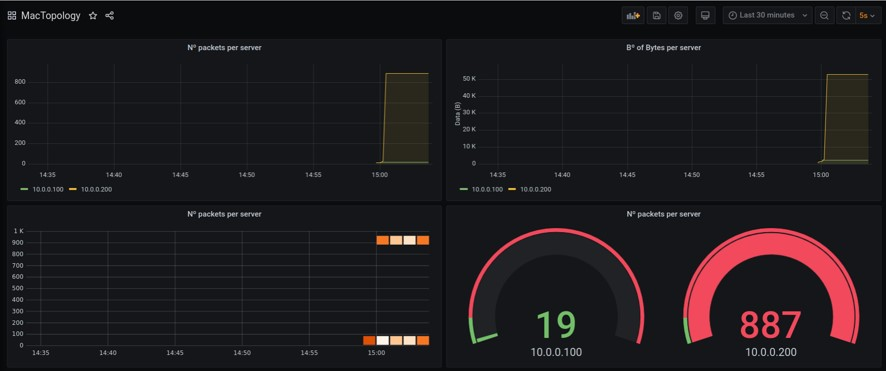
\includegraphics[width=0.9\textwidth]{grafana2.jpg}
\caption{Grafana visualization of a single attack}
\label{fig
}
\end{figure}

The next image shows two web servers each subjected to an attack at different times. It is evident that once a predefined threshold is reached, the attacker's IP address is blocked, thereby stopping the attack.

\begin{figure}[h]
\centering
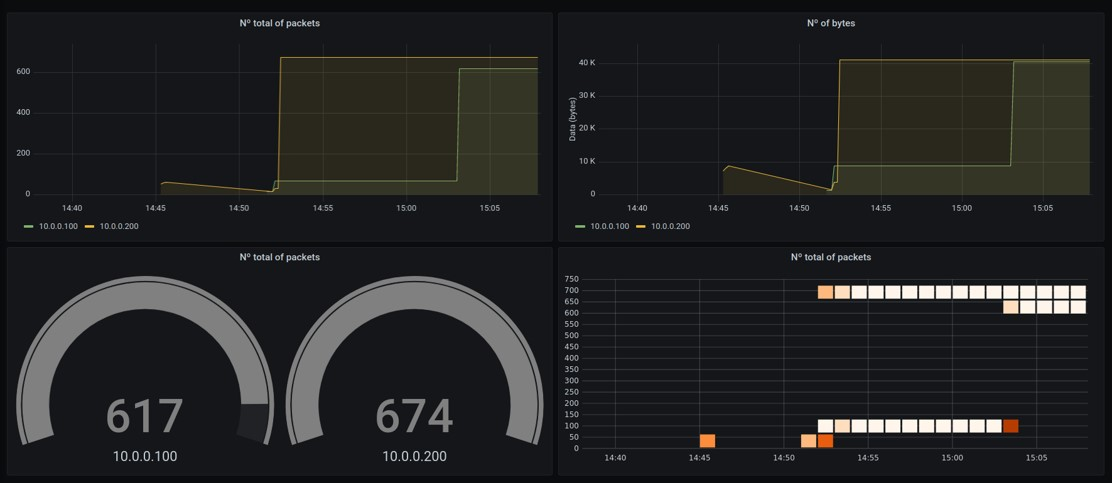
\includegraphics[width=0.9\textwidth]{grafana1.jpg}
\caption{Grafana visualization of two attacks}
\label{fig
}
\end{figure}

% Results and Analysis
\section{Results and Analysis}
\begin{itemize}
    \item Description of results obtained with load balancing.
    \item Analysis of firewall performance.
    \item Results of intrusion detection with Snort.
    \item Visualization of network metrics with Grafana.
\end{itemize}

% Discussion
\section{Discussion}
The results obtained from the implementation of the SDN project have shown significant improvements in network manageability and security. The load balancer is able to successfully grant access to services for the priority customers, even under stress from a DoS attack.
On the other hand, the firewall with snort work perfectly in conjunction to detect DoS attacks and proceed blocking the machines. Even if the machine is targeted as a regular customer.
Finally grafana is integrated for real time statistics about the load on the servers.

However, some limitations were encountered during the project. The scalability of the network was limited by the computational resources available, and certain advanced features of Snort were not fully utilized due to configuration complexities. Future work could focus on addressing these limitations by deploying the SDN in a more scalable environment and exploring additional security features. For example displaying blocked IPs or more metrics we would be interested in gathering.

Overall, this project has highlighted the practical benefits of SDN and provided valuable insights into its implementation and management.

\section{Conclusions}

The implementation of the SDN project has successfully demonstrated the benefits and capabilities of software-defined networking in a controlled environment. Using Mininet and the Ryu controller, we have integrated several critical functionalities, including load balancing, firewall rules, and network monitoring, each managed efficiently through SDN principles.

\subsection{Achievements}

The project achieved several key objectives:
\begin{itemize}
    \item \textbf{Load Balancing:} Implemented a dynamic load balancing solution that effectively distributes network traffic across multiple servers, optimizing resource utilization and reducing latency.
    \item \textbf{Security Enhancements:} Deployed a robust firewall system using the Ryu controller's REST API, allowing dynamic and flexible rule management to protect the network from unauthorized access.
    \item \textbf{Intrusion Detection:} Integrated Snort IDS with the SDN to monitor network traffic in real-time, detecting and responding to potential security threats promptly.
    \item \textbf{Performance Monitoring:} Established a comprehensive monitoring framework with Telegraf and Grafana, providing real-time visualization of network performance metrics such as bandwidth usage, latency, and packet loss.
\end{itemize}

\subsection{Challenges and Limitations}

While the project was successful in many aspects, several challenges and limitations were encountered:
\begin{itemize}
    \item \textbf{Scalability:} The network's scalability was limited by the computational resources available in the simulation environment. Deploying the SDN in a real-world, large-scale environment could present additional challenges.
    \item \textbf{Complexity of Integration:} Integrating various tools like Snort, Telegraf, and Grafana required careful configuration and troubleshooting, which can be complex and time-consuming.
    \item \textbf{Advanced Features Utilization:} Certain advanced features of Snort and other tools were not fully utilized due to configuration complexities and time constraints.
\end{itemize}

\subsection{Lessons Learned}

Throughout the project, several valuable lessons were learned:
\begin{itemize}
    \item \textbf{Importance of Documentation:} Comprehensive documentation of each component and its configuration is crucial for effective integration and troubleshooting.
    \item \textbf{Modular Design:} Designing the network and its components in a modular fashion helps in managing complexity and allows for easier testing and debugging.
    \item \textbf{Continuous Monitoring:} Implementing continuous monitoring and real-time visualization is essential for maintaining network health and quickly identifying and resolving issues.
\end{itemize}

\subsection{Future Work}

Based on the findings and limitations identified, several areas for future work are proposed:
\begin{itemize}
    \item \textbf{Enhanced Scalability:} Deploying the SDN in a cloud-based environment or on physical hardware to test its scalability and performance under real-world conditions.
    \item \textbf{Improved Security Measures:} Integrating more advanced security measures, such as machine learning-based anomaly detection and automated response mechanisms.
    \item \textbf{Extended Monitoring Capabilities:} Expanding the monitoring framework to include more detailed metrics and using predictive analytics to anticipate and mitigate potential issues.
    \item \textbf{Controller Performance Evaluation:} Exploring the use of other SDN controllers, such as OpenDaylight or ONOS, and comparing their performance, scalability, and feature sets with Ryu.
    \item \textbf{Automated Configuration Management:} Implementing automated configuration management tools to streamline the setup and maintenance of the SDN and its integrated components.
    \item \textbf{Broader Attack Detection and Mitigation:} Extending the current work beyond DoS attacks to detect and mitigate other types of cyber-attacks such as Distributed Denial of Service (DDoS), brute force attacks, and other sophisticated attack vectors. This could involve the development and integration of new detection algorithms and mitigation strategies tailored to these threats.
\end{itemize}

In conclusion, the project has successfully showcased the potential of software-defined networking in enhancing network flexibility, security, and performance monitoring. The integration of various tools and functionalities demonstrates the versatility and effectiveness of SDN in managing modern network infrastructures. Further research and development in the areas identified can lead to even more robust and scalable SDN solutions.




% Appendices
\section{Source Code}

The complete source code for this project is available on GitHub. You can access it using the following link:

\begin{quote}
\url{https://github.com/oriolmiranda/SDS_project}
\end{quote}

The repository includes all the scripts used in the project, such as:

\begin{itemize}
    \item \texttt{snort.py} - Integrates Snort IDS with the Ryu controller.
    \item \texttt{rest\_firewall.py} - Implements a firewall using the Ryu controller.
    \item \texttt{load\_balancer.py} - Manages load balancing across multiple servers.
    \item \texttt{monitor\_telegraf.py} - Collects and visualizes network performance metrics using Telegraf and Grafana.
    \item \texttt{initialize.sh} - A shell script that sets up the environment and cleans.
    \item \texttt{macTopology.py} - Defines the structure of the network simulated in Mininet, including the switches, hosts, and links needed for testing and development of network applications.
    \item \texttt{rules\_firewall.sh} - Contains the firewall rules that apply to the network, defining security policies to control traffic and protect the network infrastructure.
\end{itemize}

Please visit the repository to explore the complete implementation details and to download the code.

% References
\begin{thebibliography}{9}
\bibitem{mininet} Mininet: An Instant Virtual Network on your Laptop (or other PC). \url{http://mininet.org/}
\bibitem{ryu} Ryu SDN Framework. \url{https://osrg.github.io/ryu/}
\bibitem{snort} Snort: The Open Source Network Intrusion Detection System. \url{https://www.snort.org/}
\end{thebibliography}

\end{document}